\paragraph{} A codificação de Huffman é um método de compressão que consiste em encontrar uma representação alternativa --- um \emph{código} --- para cada \emph{símbolo} do alfabeto dos dados a comprimir. A compressão resulta do facto de o código escolhido para um dado símbolo ser tanto mais curto quanto maior for a frequência absoluta desse símbolo nos dados. A símbolos mais raros são atribuídos códigos mais longos. Os códigos encontrados têm uma propriedade importante: nenhum código é prefixo de outro código. Isto permite que durante o processo de descompressão não haja qualquer ambiguidade.

Os passos necessários ao algoritmo de compressão são os seguintes:

\begin{enumerate}
  \item obter as frequências absolutas de cada símbolo
  \item construir uma árvore de Huffman
  \item codificar os dados
\end{enumerate}

O primeiro passo consiste em contar o número de ocorrências de cada símbolo até encontrar o fim do ficheiro. O segundo passo é criar uma \emph{trie} a partir das frequências obtidas no primeiro passo. Por último o ficheiro é comprimido fazendo uso da árvore criada.

O processo de criação da árvore de Huffman é:

\begin{enumerate}
  \item criar um nó para cada símbolo do alfabeto, em que se inclui a frequência desse símbolo
  \item enquanto existir mais que uma árvore
    \begin{enumerate}
    \item encontrar as duas árvores cuja raiz tem menor frequência
    \item tornar essas árvores descendentes de um novo nó, cuja frequência é a soma das frequências das raízes das duas árvores
  \end{enumerate}
\end{enumerate}

No final sobra apenas uma árvore que contém os nós correspondentes a cada símbolo. A localização desses nós na \textit{trie} dá-nos o código desse símbolo.

\subsection*{Exemplo}

\paragraph{} Tome-se como exemplo o ficheiro \texttt{ABBCCCDDDD<EOF>}, em que \texttt{<EOF>} é o carácter terminador do ficheiro. As estatísticas do ficheiro são as seguintes: \texttt{\{A: 1, B: 2, C: 3, D: 4, <EOF>: 1\}}. A partir das estatísticas retiradas do ficheiro é gerada uma lista de prioridade. Na \autoref{fig:prio_list} apresenta-se a lista obtida.

\begin{figure}[H]
  \centering
  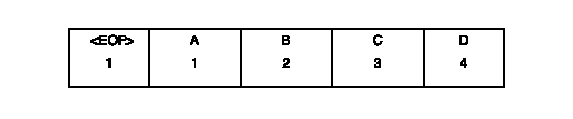
\includegraphics[width=.65\textwidth]{img/prio_list}
  \caption{Lista de prioridade gerada a partir das estatísticas}
  \label{fig:prio_list}
\end{figure}

De seguida retira-se os 2 elementos de menor prioridade da lista - neste caso \texttt{A} e \texttt{<EOF>} - e cria-se um novo nó que guarda a soma das suas frequências.

\begin{figure}[H]
  \centering
  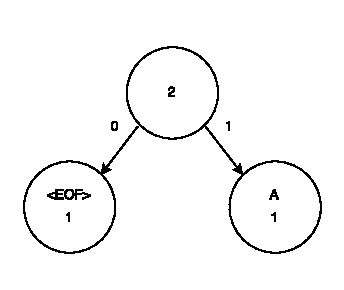
\includegraphics[width=.5\textwidth]{img/trie_1}
  \caption{Primeiro nó da árvore}
  \label{fig:trie_1}
\end{figure}

O novo nó vai ser adicionado à lista de prioridades, chamando-se \texttt{Nó 1}.

\begin{figure}[H]
  \centering
  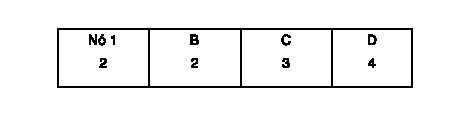
\includegraphics[width=.65\textwidth]{img/prio_list_2}
  \caption{Lista de prioridade com \texttt{Nó 1} adicionado}
  \label{fig:prio_list_2}
\end{figure}

Este processo repete-se até só existir um elemento na lista de prioridade. Na \autoref{fig:final_huffman_tree_example} encontra-se a árvore de Huffman final criada para este ficheiro.

\begin{figure}[H]
  \centering
  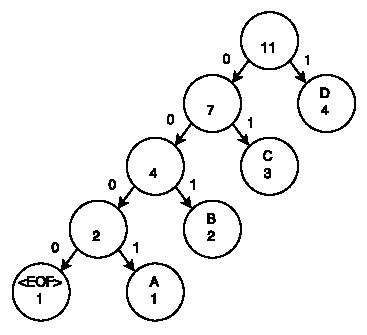
\includegraphics[width=.65\textwidth]{img/huffman_tree_example}
  \caption{Exemplo de uma árvore de Huffman}
  \label{fig:final_huffman_tree_example}
\end{figure}

Os códigos para cada carácter obtêm-se percorrendo a \textit{trie} da raiz até à folha que contem o respectivo carácter. Cada vez que se passa para um filho à esquerda adiciona-se o bit 0 à codificação; cada vez que se segue para um filho à direita adiciona-se um bit com o valor 1. Assim, por exemplo o código de \texttt{A} é \texttt{0001}, o de \texttt{C} é \texttt{01} e o de \texttt{D} é \texttt{1}. É de notar que, tal como previsto, os caracteres que ocorrem menos vezes têm códigos mais curtos.

O ficheiro comprimido seria portanto \texttt{0001 001 001 01 01 01 1 0000}. De $11 \times 8 = 88$ bits - assumindo que é usada a representação ASCII - passou-se a 21 bits.

No entanto, seria ainda necessário colocar no ficheiro uma representação da árvore para que o ficheiro pudesse ser descomprimido. A árvore poderia ser representada no ficheiro de saída como \texttt{00001 <EOF> 1 A 1 B 1 C 1 D}, em que \texttt{A}, \texttt{B}, \texttt{C}, \texttt{D} e \texttt{<EOF>} representam a codificação original do caracteres em ASCII. Assim, na realidade o ficheiro comprimido teria neste caso $21 + 9 + 5 \times 8 = 70$ bits, obtendo-se um rácio de compressão de $79,5\%$. Em ficheiros pequenos a inclusão da árvore tem um grande impacto, como se percebe por este exemplo. Em ficheiros grandes o \textit{overhead} da inclusão da árvore é desprezável.
